% Section content template for individual Educative lessons
% This file contains the actual content for a specific section
% Generated from Educative API section content

% Section: Detailed Design of WhatsApp
% Section ID: 6731604231192576
% Section Slug: detailed-design-of-whatsapp
% Generated: 2025-12-08T15:00:42.002758

\subsection{Detailed design}\label{Rq5YKC46WsJFtaM9iQSac}
\\
The high-level design discussed in the previous lesson doesn't answer the following questions:

\begin{itemize}
\item
\protect\phantomsection\label{QMgIhUenhpdQNpCwoww-4}
How is a communication channel created between clients and servers?
\item
\protect\phantomsection\label{of2Sde2VeQY7hnWvhOynh}
How can the high-level design be scaled to support billions of users?
\item
\protect\phantomsection\label{Avmm2XXX8yAdYij4wPlbX}
How is the user's data stored?
\item
\protect\phantomsection\label{4go97-LnkJUmeSXnc4xJ3}
How is the receiver identified to whom the message is delivered?
\end{itemize}
\\
To answer all these questions, let's dive deep into the high-level design and explore each component in detail. Let 's start with how users make connections with the chat servers.

\subsubsection{Connection with a WebSocket server}\label{B5B1o_aVayCnSRGLokV2u}
\\
In WhatsApp, each active device is connected with a \textbf{WebSocket server} via WebSocket protocol. A WebSocket server keeps the connection open with all the active (online) users. Since one server isn't enough to handle billions of devices, there should be enough servers to handle billions of users. The responsibility of each of these servers is to provide a port to every online user. The mapping between servers, ports, and users is stored in the WebSocket manager that resides on top of a cluster of the data store. In this case, that's Redis.

\begin{figure}[htbp]
 \centering
 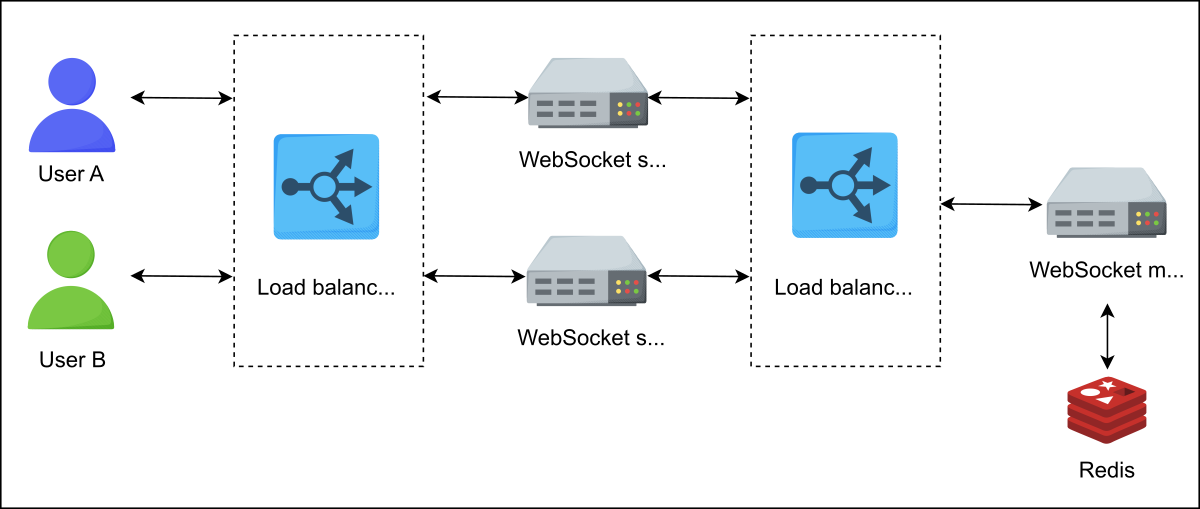
\includegraphics[width=0.5\textwidth]{Images/chapter_36/section_6731604231192576/4698647113891840.png}
 \caption{Two users are connected via WebSocket handlers}
\end{figure}

\begin{quote}
\textbf{Quiz:}
\textbf{Question 1:} Why is WebSocket preferred over HTTP(S) protocol for client-server communication?
\textbf{Answer:} HTTP(S) doesn't keep the connection open for the servers to send frequent data to a client. With HTTP(S) protocol, a client constantly requests updates from the server, commonly called polling, which is resource intensive and causes latency. WebSocket maintains a persistent connection between the client and a server. This protocol transfers data to the client immediately whenever it becomes available. It provides a bidirectional connection used as a common solution to send asynchronous updates from a server to a client.
\end{quote}

\subsubsection{Send or receive messages}\label{z7W_XbJvyLHwlZCyjWJEf}
\\
The WebSocket manager is responsible for maintaining a mapping between an active user and a port assigned to the user. Whenever a user is connected to another WebSocket server, this information will be updated in the data store.
\\
A WebSocket server also communicates with another service called message service. \textbf{Message service} is a repository of messages on top of the Mnesia database clusterMnesia. It acts as an interface to the Mnesia database for other services interacting with the databases. It is responsible for storing and retrieving messages from the Mnesia database. It also deletes messages from the Mnesia database after a configurable amount of time. And, it exposes APIs to receive messages by various filters, such as user ID, message ID, and so on.

\begin{figure}[htbp]
 \centering
 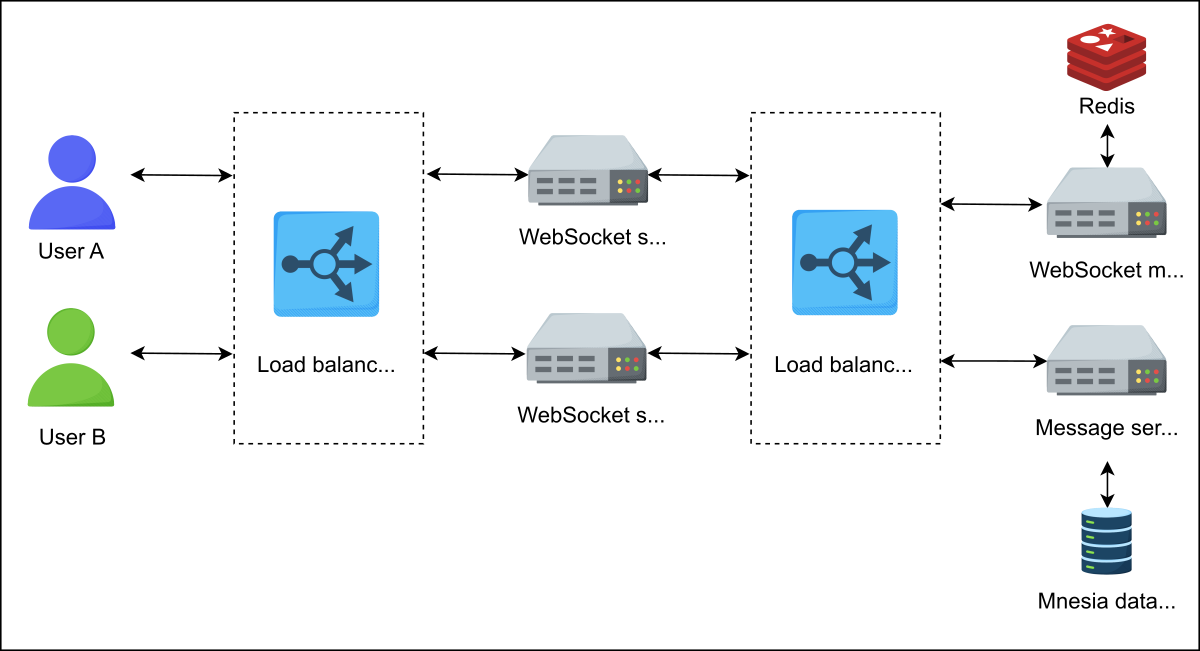
\includegraphics[width=0.5\textwidth]{Images/chapter_36/section_6731604231192576/5593304186355712.png}
 \caption{WebSocket communicates with message service on top of Mnesia database cluster}
\end{figure}

Now, let's assume that user A wants to send a message to user B. As shown in the above figure, both users are connected to different WebSocket servers. The system performs the following steps to send messages from user A to user B:

\begin{enumerate}
\item
\protect\phantomsection\label{C739fo-IAtOG1oFt_tjcR}
User A communicates with the corresponding WebSocket server to which it is connected.
\item
\protect\phantomsection\label{_PSV7VzHk0OqEjOfinwVC}
The WebSocket server associated with user A identifies the WebSocket to which user B is connected via the WebSocket manager. If user B is online, the WebSocket manager responds back to user A's WebSocket server that user B is connected with its WebSocket server.
\item
\protect\phantomsection\label{S0lsF3dHKajijaF1qMew1}
Simultaneously, the WebSocket server sends the message to the message service and is stored in the Mnesia database where it gets processed in the first-in-first-out order. As soon as these messages are delivered to the receiver, they are deleted from the database.
\item
\protect\phantomsection\label{l3JiqlomLu5LZ5iea5fM5}
Now, user A's WebSocket server has the information that user B is connected with its own WebSocket server. The communication between user A and user B gets started via their WebSocket servers.
\item
\protect\phantomsection\label{BIblNs8warpGChgVEm0tO}
If user B is offline, messages are kept in the Mnesia database. Whenever they become online, all the messages intended for user B are delivered via push notification. Otherwise , these messages are deleted permanently after 30 days.
\end{enumerate}
\\
Both users (sender and receiver) communicate with the WebSocket manager to find each other's WebSocket server. Consider a case where there can be a continuous conversation between both users. This way, many calls are made to the WebSocket manager. To minimize the latency and reduce the number of these calls to the WebSocket manager, each WebSocket server caches the following information:

\begin{itemize}
\item
\protect\phantomsection\label{UF8dDofR_ouBJHLFxPYLa}
If both users are connected to the same server, the call to the WebSocket manager is avoided.
\item
\protect\phantomsection\label{TUIDQKWF5EbCAZBn73DpU}
It caches information of recent conversations about which user is connected to which WebSocket server.
\end{itemize}

\begin{quote}
\textbf{Quiz:}
\textbf{Question 1:} The data in the cache will become outdated if a user gets disconnected and connects with another server. Keeping this in mind, how long should a WebSocket server cache information?
\textbf{Answer:} The information will be updated in the WebSocket manager when a user disconnects due to some faults in the connection and reconnects with a different WebSocket server. The WebSocket manager, in turn, invalidates the data in the cache used by the WebSocket servers, and the updated data is sent to the corresponding cache. So, the information in the cache will remain there until it receives an invalidate signal from the

WebSocket manager.
\end{quote}

\subsubsection{Send or receive media files}\label{IYcZ4dhApBmJUiHtg_SYZ}
\\
So far, we've discussed the communication of text messages. But what happens when a user sends media files? Usually, the WebSocket servers are lightweight and don't support heavy logic such as handling the sending and receiving of media files. We have another service called the \textbf{asset service}, which is responsible for sending and receiving media files.
\\
Moreover, the sending of media files consists of the following steps:

\begin{enumerate}
\item
\protect\phantomsection\label{4uS_B_80wzSlJExzbqzF5}
The media file is compressed and encrypted on the device side.
\item
\protect\phantomsection\label{hBQd4y31eId1uWdVba0Fl}
The compressed and encrypted file is sent to the asset service to store the file on blob storage. The asset service assigns an ID that's communicated with the sender. The asset service also maintains a hash for each file to avoid duplication of content on the blob storage. For example, if a user wants to upload an image that's already there in the blob storage, the image won't be uploaded. Instead , the same ID is forwarded to the receiver.
\item
\protect\phantomsection\label{JQnW4AxD4TRkM95QHdXSD}
The asset service sends the ID of media files to the receiver via the message service. The receiver downloads the media file from the blob storage using the ID.
\item
\protect\phantomsection\label{3LhSIpjDFkL1UvZ52bbww}
The content is loaded onto a CDN if the asset service receives a large number of requests for some particular content.
\end{enumerate}
\\
The following figure demonstrates the components involved in sharing media files over WhatsApp messenger:

\begin{figure}[htbp]
 \centering
 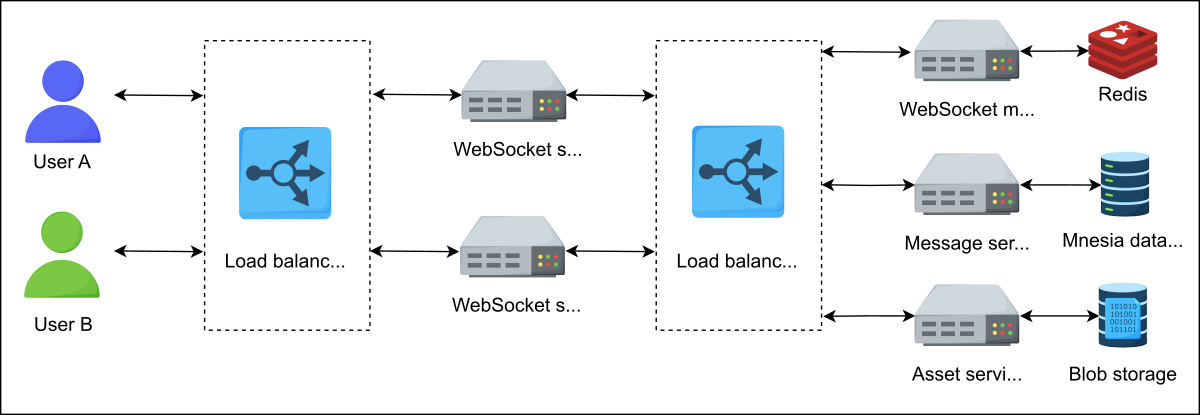
\includegraphics[width=0.5\textwidth]{Images/chapter_36/section_6731604231192576/5497257023897600.png}
 \caption{Sending media files via the asset service}
\end{figure}

\subsubsection{Support for group messages}\label{2v4kk4XXe_ox6ipskAFKp}
\\
WebSocket servers don't keep track of groups because they only track active users. However, some users could be online and others could be offline in a group. For group messages, the following three main components are responsible for delivering messages to each user in a group:

\begin{itemize}
\item
\protect\phantomsection\label{mpYFHNpUom167FpAwbH6K}
Group message handler
\item
\protect\phantomsection\label{-2xQahqzng05ElMFxdy-X}
Group message service
\item
\protect\phantomsection\label{s5GzE009-fUm7Ln5j22hj}
Kafka
\end{itemize}
\\
Let's assume that user A wants to send a message to a group with some unique ID---for example, \texttt{Group/A}. The following steps explain the flow of a message sent to a group:

\begin{enumerate}
\item
\protect\phantomsection\label{I9NZ49X68ApekfhFAJvAT}
Since user A is connected to a WebSocket server, it sends a message to the message service intended for \texttt{Group/A}.
\item
\protect\phantomsection\label{Jb6Mx4l6T-2D__dBHwSaV}
The message service sends the message to Kafka with other specific information about the group. The message is saved there for further processing. In Kafka terminology, a group can be a topic, and the senders and receivers can be producers and consumers, respectively.
\item
\protect\phantomsection\label{Ulbn4DLmJZCYLa6cBAbhX}
Now, here comes the responsibility of the group service. The \textbf{group service} keeps all information about users in each group in the system. It has all the information about each group, including user IDs, group ID, status, group icon, number of users, and so on. This service resides on top of the MySQL database cluster, with multiple secondary replicas distributed geographically. A Redis cache server also exists to cache data from the MySQL servers. Both geographically distributed replicas and Redis cache aid in reducing latency.
\item
\protect\phantomsection\label{svk8ZPRzGeh61TXdLAN7G}
The group message handler communicates with the group service to retrieve data of \texttt{Group/A} users.
\item
\protect\phantomsection\label{sb8DdCn2QLLGzwcSXSI2n}
In the last step, the group message handler follows the same process as a WebSocket server and delivers the message to each user.
\end{enumerate}

\begin{figure}[htbp]
 \centering
 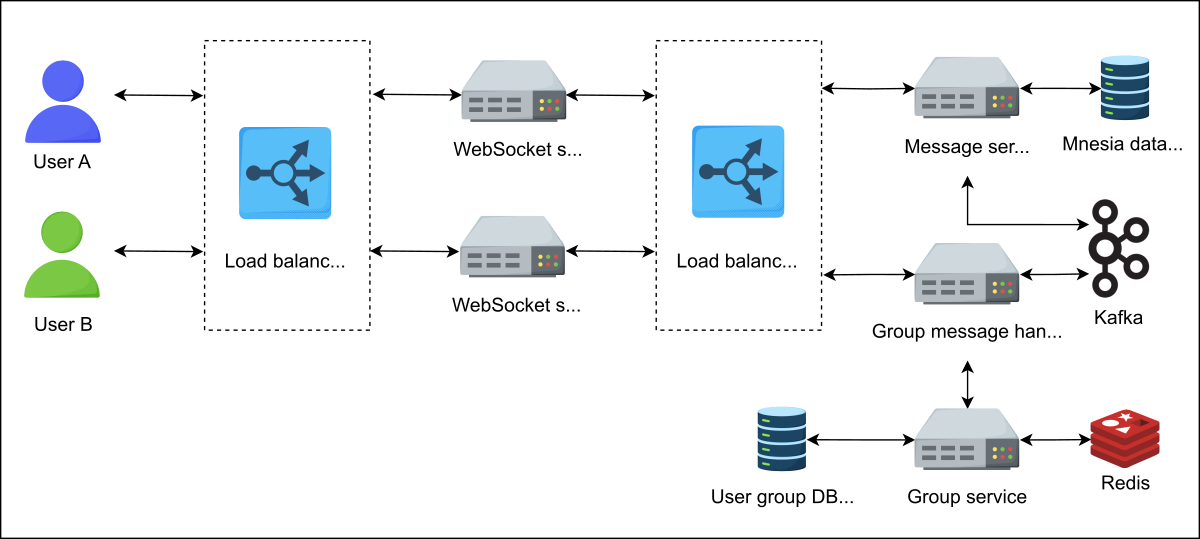
\includegraphics[width=0.5\textwidth]{Images/chapter_36/section_6731604231192576/5773445667618816.png}
 \caption{Components responsible for sending group messages}
\end{figure}

\subsubsection{End-to-end encryption}\label{end-to-end-encryption}
\\
Similar to the group message service, there's another service known as \textbf{user service} that keeps track of each user. It contains user-related data, such as name, profile picture, status, and so on. This service resides on top of the MySQL database and utilizes cache for frequently used data.
\\
At registration time, a WhatsApp client generates a number of public-private key pairs that include keys pairs for identity, a signed prekey, and a batch of one-time prekeys. These keys are used for different purposes. The public keys are stored in the database associated with the user service along with the user's identifier. Whenever a sender wants to establish a connection with the receiver, it also requests the server for the keys associated with a receiver's ID. Private keys are only stored on the client's end devices.
\\
\paragraph{One-to-one communication}\label{one-to-one-communication}
\\
To communicate securely, WhatsApp clients, on both sender and receiver sides, establish a pairwise encrypted session with each other. The session is created using the following steps:

\begin{enumerate}
\def\labelenumi{\arabic{enumi}.}
\item
The sender requests the public identity key, signed prekey, and a single public one-time prekey of the receiver's device. The one-time prekey is used only once.
\item
The WhatsApp server returns the requested public keys of the receiver.
\item
The sender generates an ephemeral Curve25519 key pair.
\item
The sender creates a master secret key using its own identity key, the ephemeral key pair, and the receiver's public keys.
\item
The sender uses the HMAC-based key-derivation function (HKDF) to create two other keys known as a root key and chain key from the master secret key. The sender starts sending messages to the receiver after establishing the pairwise encrypted session. The receiver creates the same session based on the information present in the header of the first receiving message.
\item
After establishing a session, an 80-byte Message\ Key is generated based on the root and chain Keys. The Message\ Key is used for encryption and authentication of messages.
\end{enumerate}
\\
\paragraph{Group communication}\label{group-communication}
\\
The communication in a WhatsApp group is handled by the same process discussed in the previous section on one-to-one communication. A sender key, used by the signaling messaging protocol, is generated and shared with each member's device of the group using the pairwise encrypted session. The messages sent to a group are encrypted using the sender key.
\\
The communication in a group is directed by Kafka, where each user in a group subscribes to the relevant topic (a group with an associated messaging queue). The messages are then delivered in a fanout messaging pattern where messages are delivered from a single sender to multiple receivers.

\subsubsection{Simultaneous maintenance of WhatsApp sessions on multiple devices}\label{simultaneous-maintenance-of-whatsapp-sessions-on-multiple-devices}
\\
Every device on WhatsApp is identified by a device identity key. If a user uses multiple devices (a primary and several other companion devices), each device identity key is stored against the user's account on the WhatsApp server. When the WhatsApp server receives a message from a user, it transmits messages multiple times to each device linked with a user's account.
\\
Similarly, each device used by a user has its own set of encryption keys. If a set of keys of one companion device is compromised, the attacker won't be able to see messages communicated with the other device.
\\
We've just touched the basics here because security is a deep topic. See the \#key\# WhatsApp security whitepaper:https://www.whatsapp.com/security/WhatsApp-Security-Whitepaper.pdf \#key\# for further details.

\subsection{Put everything together}\label{tf0vbFslV97sgv7aB4TPw}
\\
We discussed the features of our WhatsApp system design. It includes user connection with a server, sending messages and media files, group messages, and end-to-end encryption, individually. The final design of our WhatsApp messenger is as follows:

\begin{figure}[htbp]
 \centering
 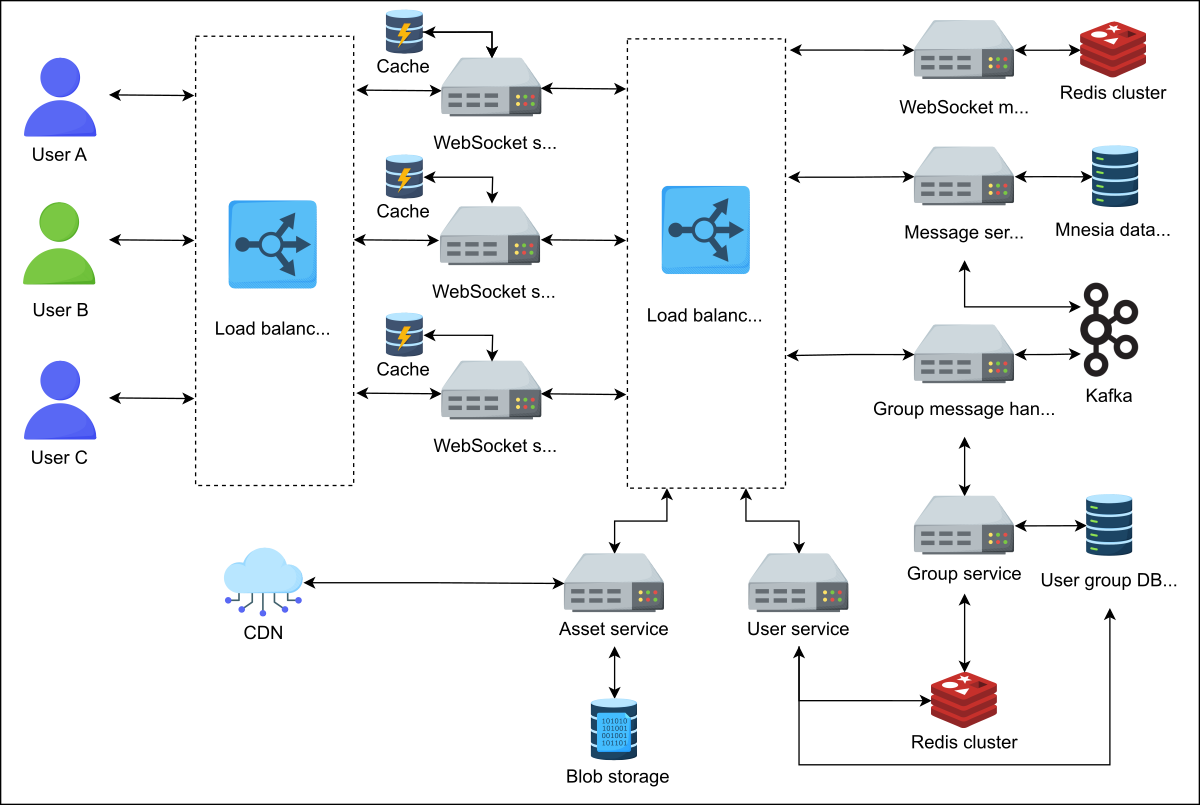
\includegraphics[width=0.5\textwidth]{Images/chapter_36/section_6731604231192576/6133792199016448.png}
 \caption{The detailed WhatsApp design. Interaction of each component with other components is shown with arrows}
\end{figure}

In the next lesson, we'll evaluate our design and look into the non-functional requirements.

% End of section content